\chapter{Discussion}
\label{chap:Discussion}
The discussion chapter will describe some of the choices made through the project and problems that have occurred. The problem and choices will be described and discussed, what happened and what could have been done differently. 

\subsubsection{Scheduling}
For the schedulability analysis, the WCET of the Arduino code had to be calculated. In the course, we learned that this could be done either with a language constructed timer, by counting clock cycles in the assembly code, or by using a tool. In our case, we used the tool Bound-T, without success. Our first idea was that a tool could provide WCET calculations for a piece of code, but because we were using libraries and loops which are not supported by Bound-T, it reported errors without a usable output. So our next idea was to calculate the WCET by analyzing the assembly code, but yet again the libraries proved to be a problem, since the source code of some libraries were inaccessible and contained unbounded loops. We tried counting the clock cycles, as shown in Appendix \ref{sec:i3Scheduling}. The next much coarser solution we tried was to estimate a worst-case running time for entire pieces of code, by using the timer implemented in the Arduino IDE. This is not a provable WCET estimate, since the odds of ever hitting the worst run time would be close to nonexistent in the little sample-size we provided. This lead to us almost doubling the WCET estimate in the UPPAAL model, as we already knew that the tasks were schedulable, even with a far greater WCET than what was estimated by the timer.

\subsubsection{Hardware choices}
To introduce other classical real-time concerns such as memory and execution time into this project, another platform smaller and slower than the Arduino Mega 2560 should’ve been chosen, since we only partly utilized the Arduino Mega 2560’s processor power. 

The two shields and their libraries for this project, the Arduino Motor Shield and the Arduino WiFi Shield, are helping us writing code to control the NXT servo motors and connecting to the network. When using both shields at the same time, some complications occurred. This is because the shields are using some of the same pins on the Arduino board. To work around this problem, it was decided to change the Arduino code such that it first connect to the network which will change a boolean to true and then initialize the motor shield components for use. This also means that it is not possible to continuously get new data from the Kinect, as it will send the first coordinate it captures and predicts of the thrown object. \newline

The motor shield should be used to control the motors, but an other solution to send the Kinect data to the arduino shield could be used. Either we should look for another WiFi component for the arduino, a bluetooth component or the robot should just be connected to the computer controlling the Kinect via a USB cable. 

As mentioned in chapter \ref{chap:Tests} about tests, the Kinect doesn’t reliably predict where the thrown object lands. In this project the depth sensor of the Kinect has been used, to calculate the impact point of the thrown object. Since the Kinect didn’t predict the impact point reliably, either the calculations made in the code should be revised or another way of using the Kinect should be taken into consideration. It is also possible that the Kinect didn’t function properly. 

Another important hardware issue in this project is the NXT servo motors. These motors capabilities severely limits the whole system’s capabilities. The motors set the boundaries of how far Dumpsty can move within a certain time limit paired with the circumference of the wheels. Having faster motors would also help on the response time of Dumpsty.


\subsubsection{Delimitations}
For this project we made two delimitations to the project, which can be found in section \ref{sec:Delimitations}. As mentioned, only one object will be thrown at any given time. This is an environmental delimitation, to not consider multiple objects at once. \newline
Another delimitation made was that the robot should not drive to coordinate points behind itself within the predefined area, but this is actually possible for the robot to do, also outside the predefined area. A problem we should have realized much earlier is that it is not possible for the robot to catch the object, unless it lands extremely close to the robot’s starting position, because of time spent processing, sending a signal and limitations of the motor. Another delimitations should have been made that the robot should not try to catch the object, but rather drive to the point where the object hit the ground. \newline
Instead the predefined area should not be considered and the robot should have a starting point at (0, 0), as shown in figure \ref{figure:discussion-graph} as the red dot. The robot should then be able to move to both of the blue crosses(direction of the old predefined area, but not limited to the old predefined area) and the green crosses behind the robot’s starting position. Meaning the robot only have a starting position at (0, 0), and the distance it can move on either axis is not limited, as it was with the predefined area. The robot should then drive to the predicted impact point of the object and just mark where the object had landed.


\begin{figure}[h]
	\centering
	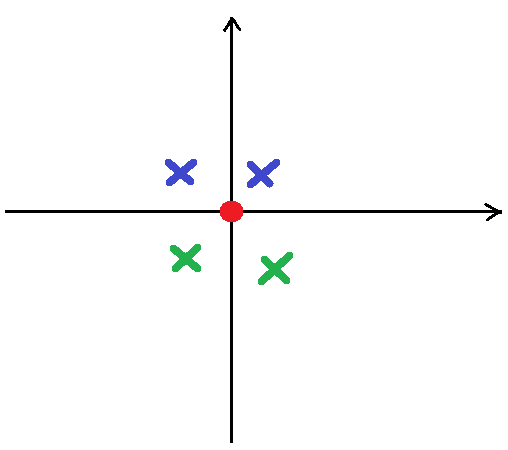
\includegraphics[scale=0.5]{billeder/discussion-graph.png}
	\caption{Graph describing the coordinate set with no predefined area}
	\label{figure:discussion-graph}
\end{figure}


\subsubsection{Process analysis}
The process model used for this project is a reflective model of the processes we have constructed our earlier projects from. This process model is based on our experience with problem based learning, and includes the processes we usually undergo through a project. It is inspired by XP, including pair programming and agile development with incrementally changing requirements. If the solution to our problem would be a safety critical solution, a more test-driven process model would be more suitable. \newline
The process model itself has worked out rather well since it isn’t restrictive and provides a very large degree of freedom when working with the project, compared to a rigid adherence to a well established model, such as the waterfall model. \newline
After experimenting with the process model throughout this project it has come to our attention that some changes should be made to the structure of the process model. A more explicit test section should be implemented to test all interdependent components, and ensure that all increments’ implementations work as intended. This will in turn also increase the coherence between each increment. This test section will also include tests across each increment, to check that no new errors has been introduced to earlier implementation.




